\section{Технологическая часть}

Данный раздел обысновывает выбор средств реализации, которые будут использоваться при разработке программного обеспечения. Будет продемонстрирован пользовательский интерфейс, как демонстрация работы программы, а также описана структура разрабатываемого программного обеспечения с помощью UML--диаграммы классов.

\subsection{Средства реализации}

Язык программирования $C++$~\cite{ISO14882_2020} выбран для разработки программного обеспечения, так как средствами языка можно реализовать разработанные алгоритмы и все необходимые типы и структуры данных, описанные в таблице~\ref{tb:types-1}, а так же из-за моего опыта работы с данным языком.

В качестве среды разработки выбрана среда $Visual~Studio~Code$~\cite{vscode}. Эта среда предоставляет набор инструментов для написания и отладки кода на различных языках программирования, включая $C++$.

\subsection{Структура программы}

На рисунке~\ref{uml} изображена структура программы в виде UML -- диаграммы.

\begin{figure}[ht!]
	\begin{center}
		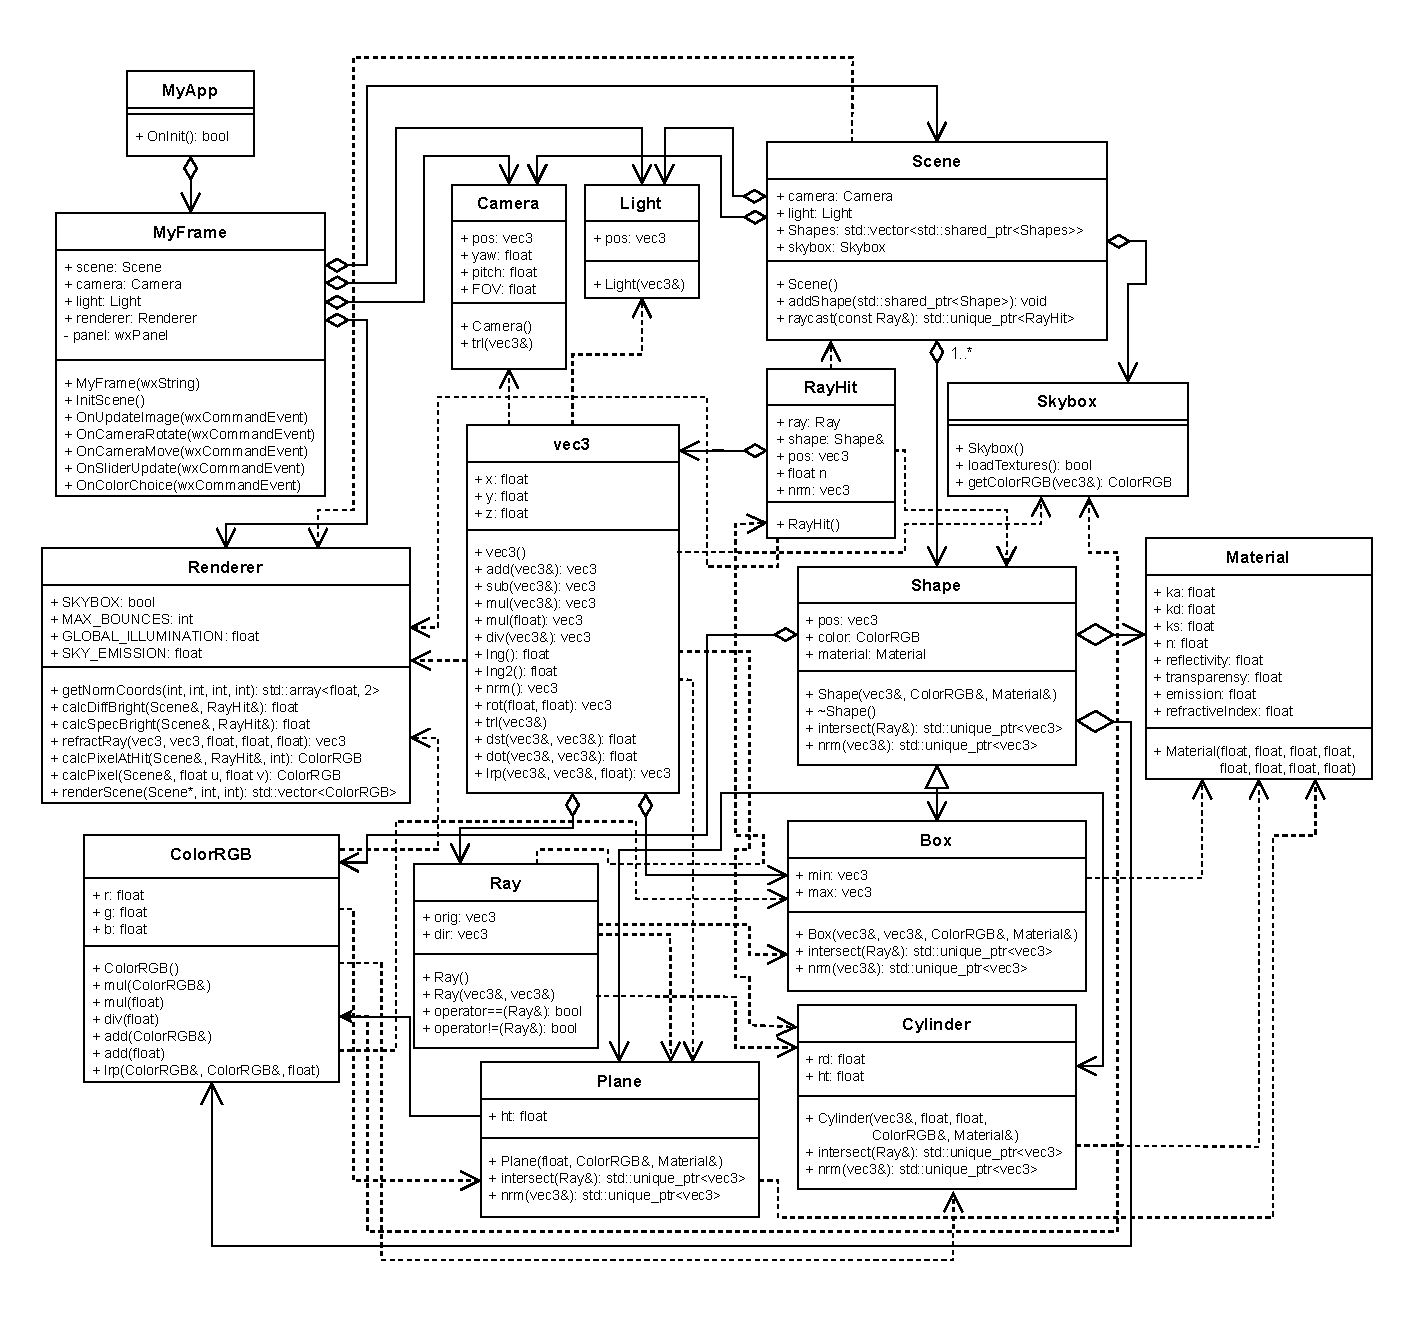
\includegraphics[scale=0.74]{diag/main-UML.pdf}
	\end{center}
	\caption{Cтруктура программы}
	\label{uml}
\end{figure}

\newpage
\subsection{Реализации алгоритмов}

На листингах~\ref{alg:1} и~\ref{alg:2} представлены реализации алгоритмов вычисления пересечения луча с цилиндром и параллелепипедом, соотвественно.

\begin{lstlisting}[label=alg:1, caption=Реализация алгоритма поиска пересечения~луча~с~цилиндром, captionpos=t]
std::unique_ptr<vec3> Cylinder::intersect(const Ray& r) const {
	vec3 intp = r.orig - pos; bool isBase = false;
	float ts1 = (ht - r.orig.y + pos.y) / (r.dir.y + EPS);
	vec3 point = intp + r.dir.mul(ts1);
	if ((point.x*point.x+point.z*point.z-rd*rd<EPS)) isBase=true;
	float ts2 = (-ht - r.orig.y + pos.y) / (r.dir.y + EPS);
	point = intp + r.dir.mul(ts2);
	if (point.x*point.x+point.z*point.z-rd*rd<EPS) isBase=true;
	float a = r.dir.x * r.dir.x + r.dir.z * r.dir.z;
	float b = r.orig.x * r.dir.x - r.dir.x * pos.x + r.orig.z * r.dir.z - r.dir.z * pos.z;
	float c = r.orig.x * r.orig.x + pos.x * pos.x + r.orig.z * r.orig.z + pos.z * pos.z - 2 * (pos.x * r.orig.x + r.orig.z * pos.z) - rd * rd;
	float delta = b * b - (a * c); float t = 0.0f;
	if (delta < EPS) { if (isBase) {
		t = std::min(ts1, ts2);
		if ((!(abs(r.orig.y+t*r.dir.y-pos.y)>ht))&&(t>0.0)) return std::make_unique<vec3>(r.orig+(r.dir.mul(t)));
	} else return nullptr; }
	float t1 = (-b-sqrt(delta))/a; float t2 = (-b+sqrt(delta))/a;
	t = (t1 < 0.0) ? t2 : t1;
	if ((!(abs(r.orig.y + t * r.dir.y - pos.y) > ht))&&(t > 0.0))
		return std::make_unique<vec3>(r.orig+(r.dir.mul(t)));
	if (!isBase) return nullptr;
	t = std::min(ts1, ts2);
	if ((!(abs(r.orig.y + t * r.dir.y - pos.y) > ht))&&(t > 0.0))
		return std::make_unique<vec3>(r.orig+(r.dir.mul(t)));
	return nullptr;
}
\end{lstlisting}

\begin{lstlisting}[label=alg:2, caption=Реализация алгоритма поиска пересечения луча с параллелепипедом, captionpos=t]
std::unique_ptr<vec3> Box::intersect(const Ray& r) const {
	float t1, t2;  float tn = -INFINITY;  float tf = INFINITY; 
	bool intersection = true;
	std::array<float, 3> rDirArr = r.dir.tArr();
	const float* rDir = rDirArr.data();
	std::array<float, 3> rayOriginArr = r.orig.tArr();
	const float* rayOrigin = rayOriginArr.data();
	std::array<float, 3> b1Arr = min.tArr();
	const float* b1 = b1Arr.data();
	std::array<float, 3> b2Arr = max.tArr();
	const float* b2 = b2Arr.data();
	for (int i = 0; i < 3; ++i) {
		if (rDir[i]==0.0f) { 
			if (rayOrigin[i]<b1[i]||rayOrigin[i]>b2[i])
				intersection = false;
		} else {
			t1=(b1[i]-rayOrigin[i])/rDir[i]; 
			t2=(b2[i]-rayOrigin[i])/rDir[i];
			if (t1 > t2) std::swap(t1, t2);
			if (t1 > tn) tn = t1; if (t2 < tf) tf = t2;
			if (tn > tf) intersection = false;
			if (tf < 0) intersection = false;
		}
	}
	return intersection ? std::make_unique<vec3>(r.orig + r.dir.mul(tn)) : nullptr;
}
\end{lstlisting}

На листинге~\ref{alg:3} представлена реализация класса $Renderer$, которая включает в себя реализации следующих алгоритмов: вычисление полного освещения для пикселя, трассировка лучей и вычисление преломления луча.

\begin{lstlisting}[label=alg:3, caption=Реализация класса $Renderer$, captionpos=t]
std::array<float, 2> Renderer::getNormCoords(int x, int y, int wt, int ht) {
	std::array<float, 2> uv;
	float u, v;
	if (wt > ht) {
		u = (x - wt / 2 + ht / 2) / static_cast<float>(ht)*2 - 1;
		v = -(y / static_cast<float>(ht) * 2 - 1);
	} else {
		u = x / static_cast<float>(wt) * 2 - 1;
		v = -((y - ht / 2 + wt / 2) / static_cast<float>(wt)*2-1);
	}
	uv[0] = u;  uv[1] = v;
	return uv;
}
vec3 Renderer::refractRay(vec3 I, vec3 n, float cos, float n1, float n2) {
	if (cos < 0.0f) return refractRay(I, n, -cos, n2, n1);
	float eta = n1/n2;
	float sin = eta * sqrtf(std::max(0.0f, 1.0f - cos * cos));
	if (sin >= 1.0f) return vec3(-1.0f, 0.0f, 0.0f); 
	return I*eta+n*(eta*cos-sqrtf(std::max(0.0f,1.0f-sin*sin)));
}
float Renderer::calcDiffBright(Scene& scene, RayHit& hit) {
	vec3 lightDir = (scene.light.pos - hit.pos).nrm();
	Ray shadowRay(hit.pos + lightDir * 0.001f, lightDir);
	auto hs = &(hit.shape); float accumulatedLight = 1.0f;
	int bounceCount = 0; float n = 1.0;
	while (bounceCount < MAX_BOUNCES) {
		++bounceCount;
		auto lightBlocker = scene.raycast(shadowRay);
		if (lightBlocker && (lightBlocker->pos - scene.light.pos).lng2() < EPS) {
			return std::max(GLOBAL_ILLUMINATION,
				std::min(1.0f, vec3::dot(hit.nrm, lightDir)) * accumulatedLight);
		}
		if (!lightBlocker) {
			return std::max(GLOBAL_ILLUMINATION,
				std::min(1.0f, vec3::dot(hit.nrm, lightDir)) * accumulatedLight);
		}
		if (&(lightBlocker->shape) == hs) {
			if (vec3::dot(lightBlocker->nrm, lightDir) > 0.0f) {
				shadowRay.orig = lightBlocker->pos + lightDir * 0.001f;
				continue;
			} else return GLOBAL_ILLUMINATION;
		}
		float transparency = (lightBlocker->shape).material.transparency * 0.9;
		if (transparency > 0.0f) {
			accumulatedLight *= transparency;
			if (accumulatedLight < 0.01f) return GLOBAL_ILLUMINATION;
			vec3 refrRay = refractRay(lightDir, lightBlocker->nrm, vec3::dot(lightDir, lightBlocker->nrm), lightBlocker->shape.material.refractiveIndex,  n);
			shadowRay.orig = lightBlocker->pos + lightDir * 0.001f;
			shadowRay.dir = refrRay.nrm();
		} else	return GLOBAL_ILLUMINATION;
		hs = &(lightBlocker->shape);
	}
	return std::max(GLOBAL_ILLUMINATION,
		std::min(1.0f, vec3::dot(hit.nrm, lightDir)) * accumulatedLight);
}
float Renderer::calcSpecBright(Scene& scene, RayHit& hit) {
	vec3 lightDir = (hit.pos - (scene.light.pos).nrm()).nrm();
	float specularFactor = std::max(0.0f, vec3::dot(lightDir - hit.nrm * (vec3::dot(lightDir, hit.nrm) * 2), 
	(scene.camera.pos - hit.pos).nrm()));
	return std::pow(specularFactor, 2.0f) * hit.shape.material.reflectivity;
}
ColorRGB Renderer::calcPixelAtHit(Scene& scene, RayHit& hit, int limit) {
	const ColorRGB hitColorRGB = hit.shape.color;
	const float dBright = calcDiffBright(scene, hit);
	const float sBright = calcSpecBright(scene, hit);
	const float reflectivity = hit.shape.material.reflectivity;
	const float emission = hit.shape.material.emission;
	const float transparency = hit.shape.material.transparency;
	const float n1 = hit.n; const float n2 = hit.shape.material.refractiveIndex;
	ColorRGB reflectionColor; ColorRGB refractionColor;
	float dirCos = vec3::dot(hit.ray.dir, hit.nrm);
	vec3 reflectRayDir = hit.ray.dir - (hit.nrm * (2.0f * dirCos));
	vec3 reflectRayOrig = hit.pos + (reflectRayDir * 0.001f);
	vec3 refractRayDir = refractRay(hit.ray.dir, hit.nrm, dirCos, n2, n1);
	vec3 refractRayOrig = hit.pos + (refractRayDir * 0.001f);
	std::unique_ptr<RayHit> reflectHit = (limit > 0) ? scene.raycast(Ray(reflectRayOrig, reflectRayDir)) : nullptr;
	if (reflectHit) reflectionColor = calcPixelAtHit(scene, *reflectHit, limit - 1);
	else if (SKYBOX) reflectionColor = scene.skybox.getColorRGB(reflectRayDir).mul(SKY_EMISSION);
	else reflectionColor = ColorRGB::SKYBLUE;
	std::unique_ptr<RayHit> refractHit = (limit > 0) ? scene.raycast(Ray(refractRayOrig, refractRayDir)) : nullptr;
	if (refractHit) refractionColor = calcPixelAtHit(scene, *refractHit, limit - 1);
	else if (SKYBOX) refractionColor = scene.skybox.getColorRGB(refractRayDir).mul(SKY_EMISSION);
	else refractionColor = ColorRGB::SKYBLUE;
	ColorRGB pixelColorRGB = ColorRGB::lrp(hitColorRGB, reflectionColor, reflectivity).mul(dBright).add(sBright).add(reflectionColor .mul(reflectivity *emission)) .add(refractionColor.mul(transparency));
	return pixelColorRGB;
}
ColorRGB Renderer::calcPixel(Scene& scene, float u, float v) {
	vec3 eyePos(0.0f, 0.0f, (-1.0f / std::tan(scene.camera.fOV * M_PI / 360.0f))); 
	Camera& cam = scene.camera;
	vec3 rayDir = (vec3(u, v, 0.0f) - eyePos).nrm().rot(cam.yaw, cam.pitch);
	auto hitPtr = scene.raycast(Ray(eyePos + cam.pos, rayDir));
	if (hitPtr) return calcPixelAtHit(scene, *hitPtr, MAX_BOUNCES);
	else if (SKYBOX) return scene.skybox.getColorRGB(rayDir).mul(SKY_EMISSION);
	else return ColorRGB::SKYBLUE;
}
std::vector<ColorRGB> Renderer::renderScene(Scene* scene, int wt, int ht) {
	std::vector<ColorRGB> pixels(wt * ht); 
	auto start = std::chrono::high_resolution_clock::now();
	int numThreads = std::thread::hardware_concurrency();
	if (numThreads == 0) numThreads = 8;
	auto renderBlock = [&scene, &pixels, wt, ht](int startX, int startY, int blockWidth, int blockHeight) {
		for (int x = startX; x < std::min(startX + blockWidth, wt); ++x) {
			for (int y = startY; y < std::min(startY + blockHeight, ht); ++y) {
				std::array<float, 2> uv = getNormCoords(x, y, wt, ht);
				ColorRGB pixel = calcPixel(*scene, uv[0], uv[1]);
				pixels[(y * wt + x)] = pixel;
			}
		}
	};
	std::vector<std::thread> threads;
	int blockWidth = (wt + numThreads - 1) / numThreads;
	for (int t = 0; t < numThreads; ++t) {
		int startX = (t % numThreads) * blockWidth; int startY = 0;
		threads.emplace_back(renderBlock, startX, startY, blockWidth, ht);
	}
	for (auto& t : threads) { t.join(); }
	auto end = std::chrono::high_resolution_clock::now();
	std::chrono::duration<double> elapsed_seconds = end - start;
	auto elapsed_ms = std::chrono::duration_cast<std::chrono::milliseconds>(end - start); 
	std::cout << "Время рендеринга: " << elapsed_seconds.count() << " секунд (" << elapsed_ms.count() << " мс)" << std::endl;
	return pixels;
}
\end{lstlisting}

\subsection{Графический интерфейс}

На рисунках~\ref{ui-set} и~\ref{ui-img} изображены окна, представляющие графический интерфейс для пользователя.

Программа предоставляет графический интерфейс: окно для настроек рендеринга изображения; окно для отображения сгенерированного изображения. При запуске все виджеты имеют значения по умолчанию. Для того, чтобы открыть окно для отображения изображения, необходимо нажать на кнопку <<Обновить изображение>>. 

С помощью окна настроек можно выполнять следующие действия: 

	\begin{itemize}
	\item изменять позицию и поворот камеры в сцене с помощью соотвествующих кнопок на панелях <<Позиция камеры>> и <<Поворот камеры>>, соотвественно;
	\item изменять позицию источника света в сцене с помощью соотвествующих полей на панели <<Параметры источника света>>;
	\item изменять цвет, отражаемость, прозрачность и коэффициент преломления для материалов таких объектов, как сосуд и жидкость, с помощью соответствующих ползнуков и выпадающих списков на панелях <<Параметры жидкости>> и <<Параметры сосуда>>;
	\item изменять отражаемость и цвет материала для объекта -- стерженя с помощью соответствующих ползнука и выпадающего списка на панели <<Параметры стержня>>;
	\item изменять дополнительные параметры для рендеринга изображения на панели <<Дополнительные параметры>>;
	\item сгенерировать и обновить изображение для отображения с помощью кнопки <<Обновить изображение>>.
\end{itemize}

\begin{figure}[ht!]
	\begin{center}
		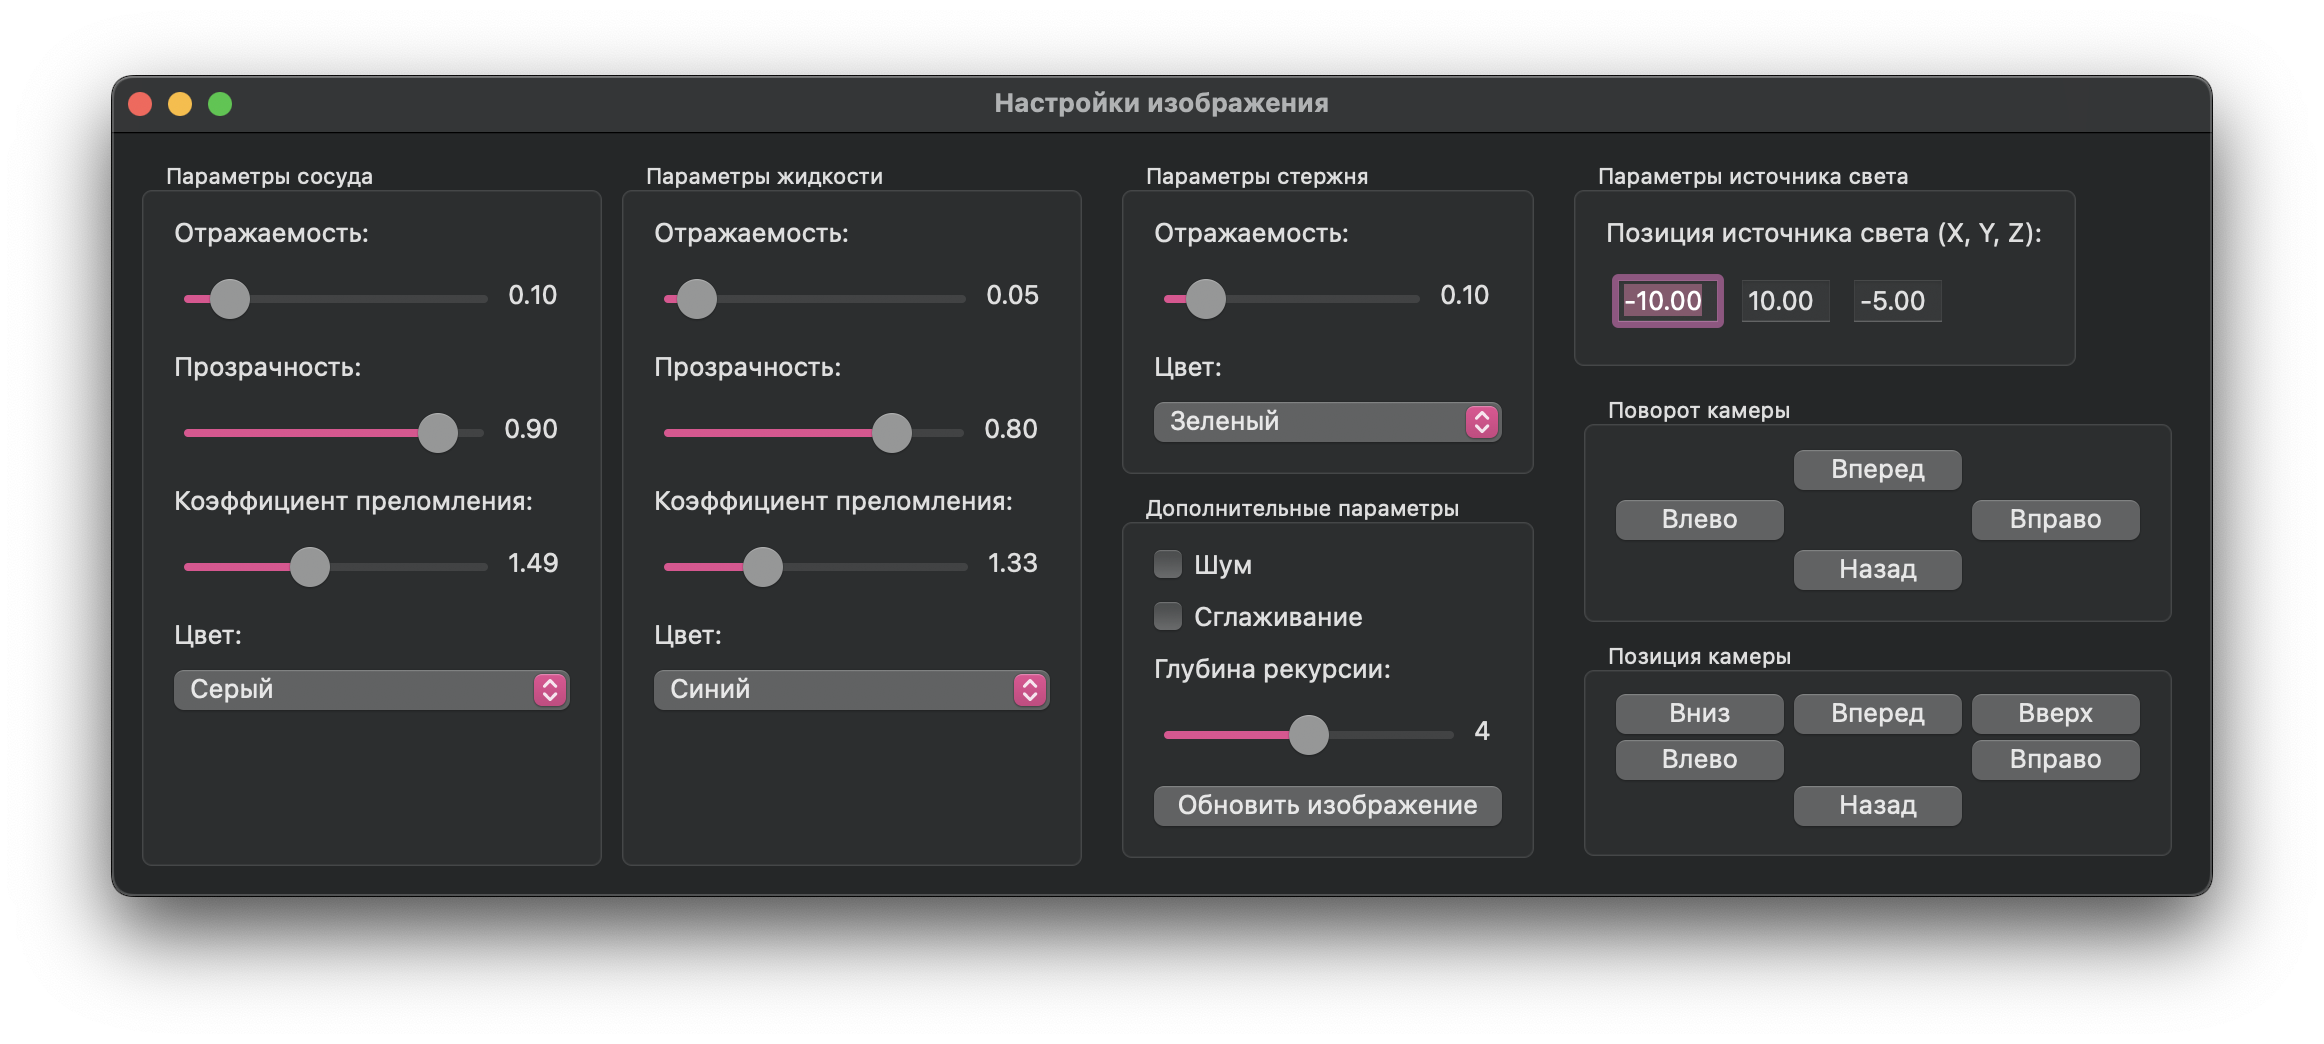
\includegraphics[scale=0.43]{img/ui-settings.png}
	\end{center}
	\caption{Пользовательский интерфейс: окно для настроек рендеринга}
	\label{ui-set}
\end{figure}

\newpage
\begin{figure}[ht!]
	\begin{center}
		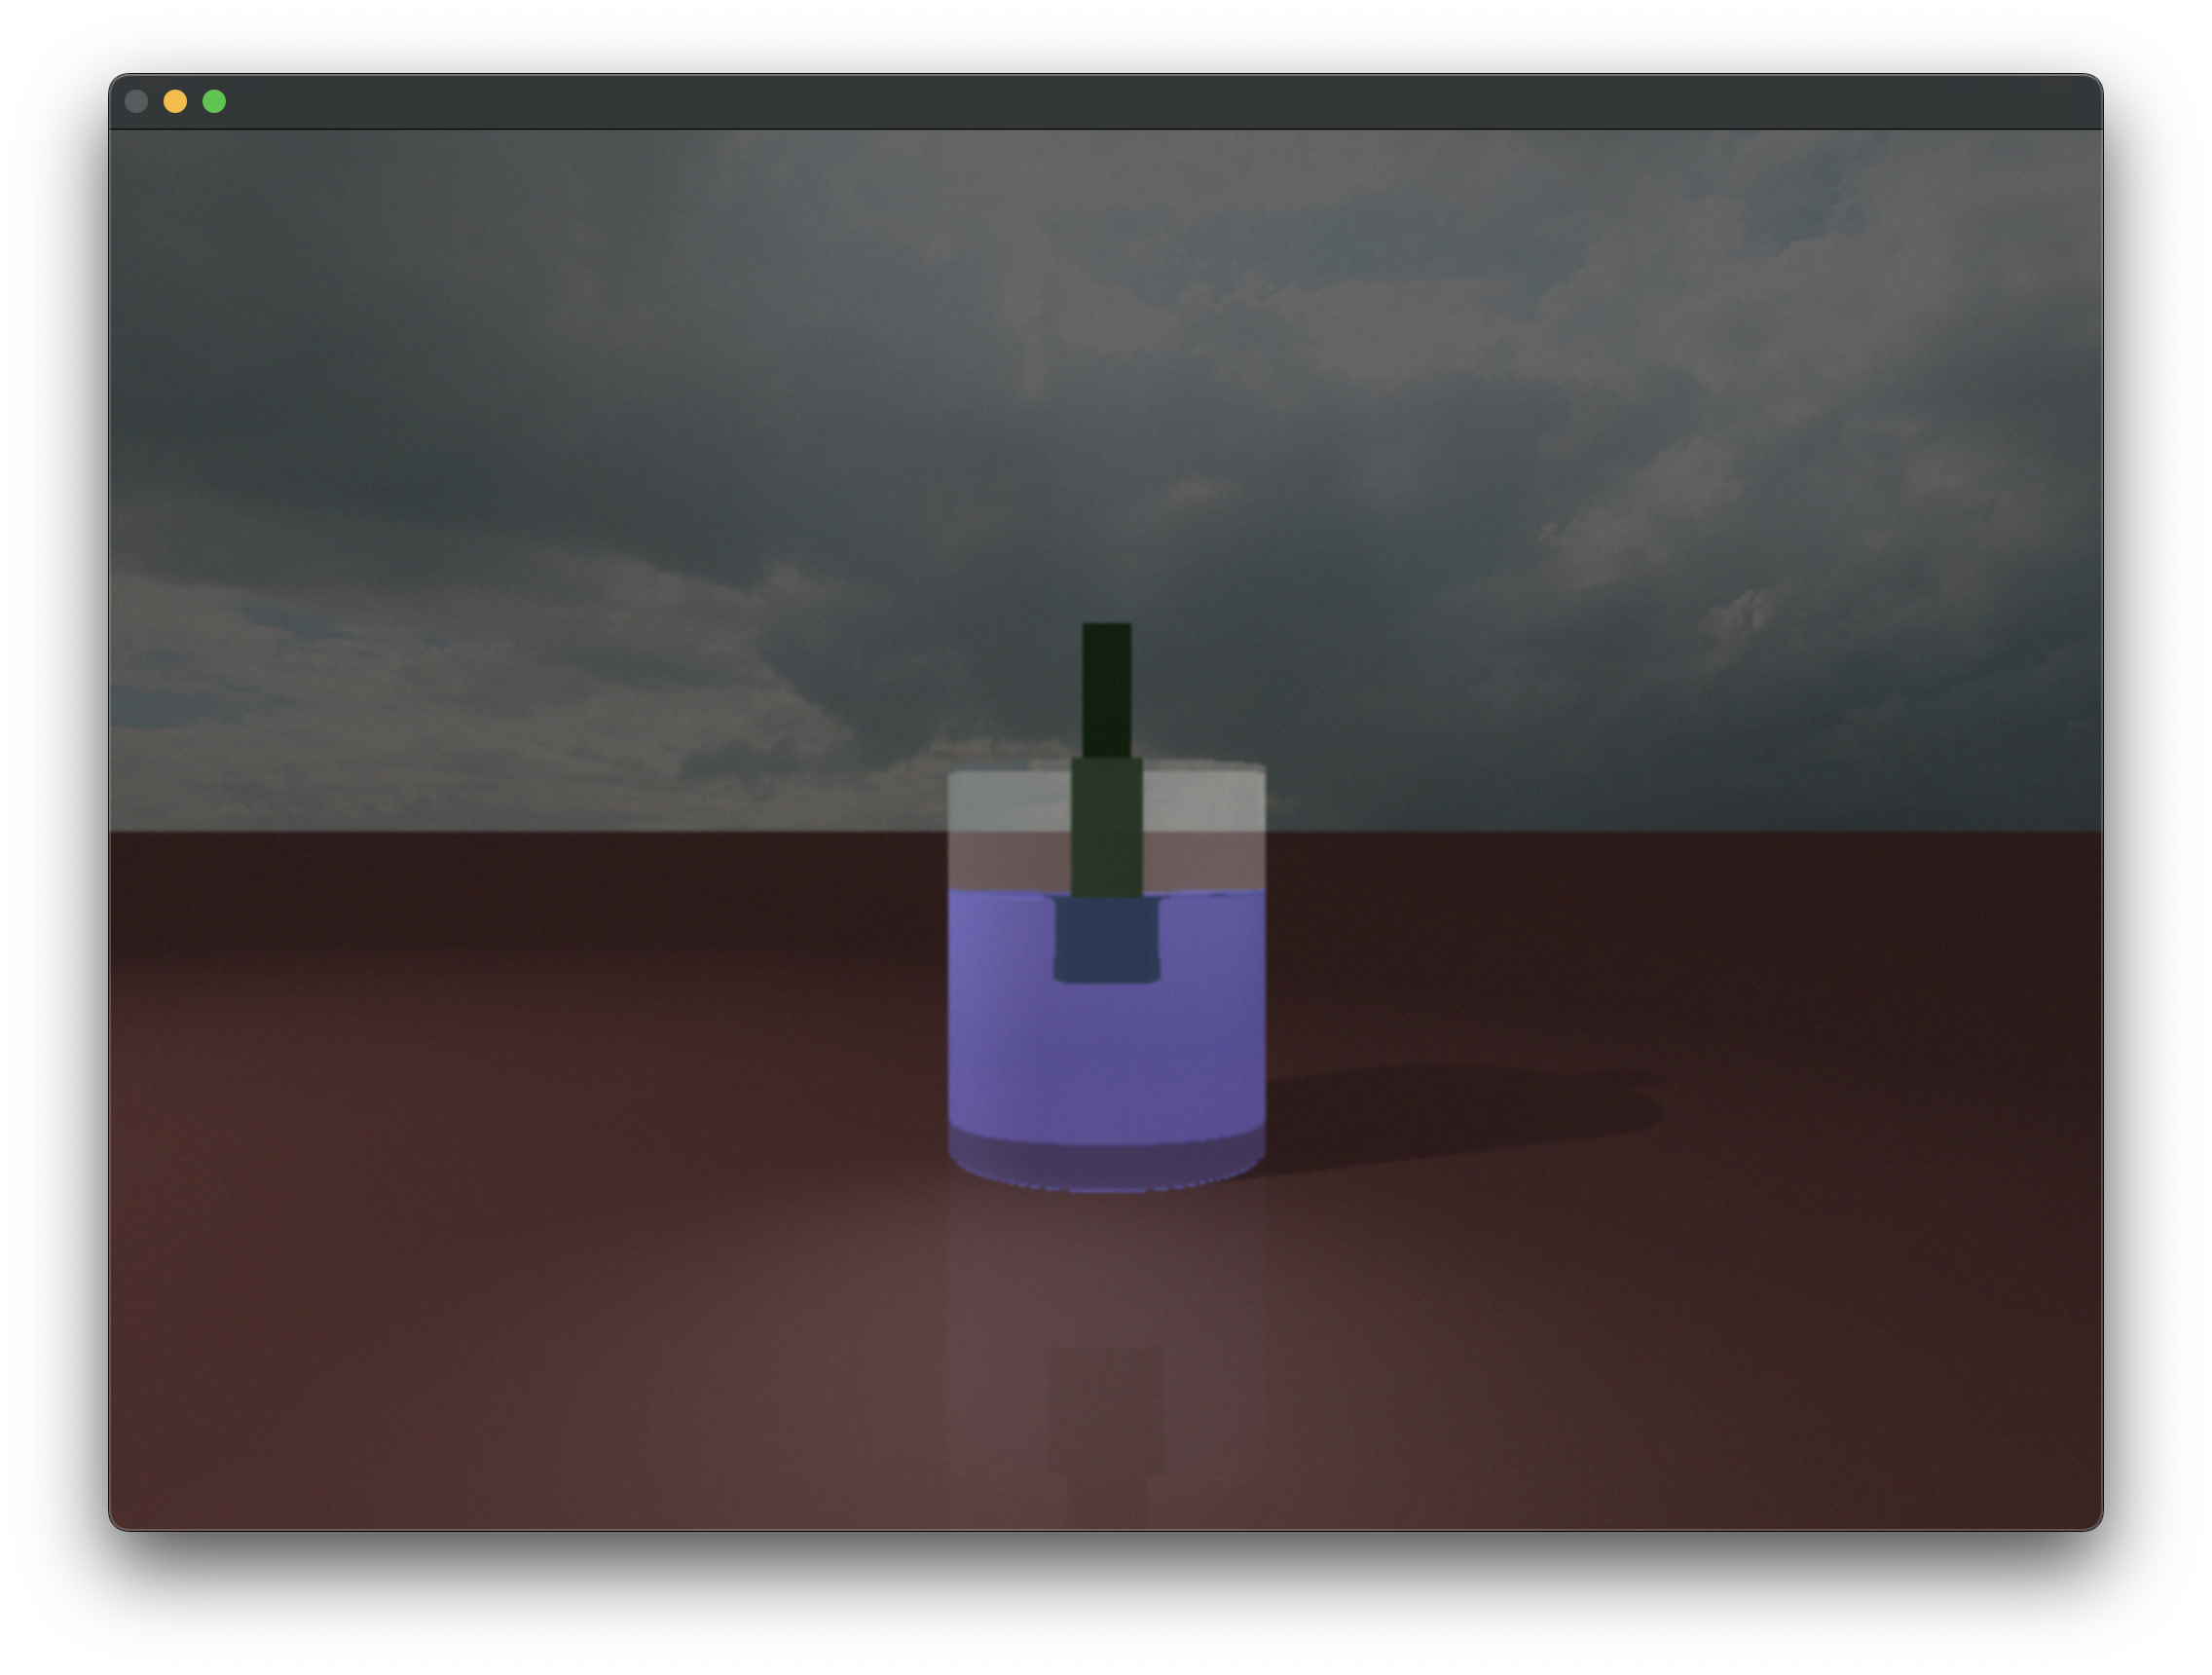
\includegraphics[scale=0.43]{img/ui-image.png}
	\end{center}
	\caption{Пользовательский интерфейс: окно для отображения изображения}
	\label{ui-img}
\end{figure}

\subsection*{Вывод}

В данном разделе были выбраны средства реализации для программного обеспечения, привидена структура программы в виде UML -- диаграммы классов, и предоставлены реализации разработанных алгоритмов. Также описан графический интерфейс, и приведена демонстрация работы программы.